Benchmarking-delens fremmeste formål er at finde svar på en række spørgsmål
inden udregningen sættes igang. Vi præsenterer her resultaterne af en lang række prøvekørsler, hver med en kort beskrivelse af omstændigheder omkring kørslen og de udledninger vi har foretaget på baggrund af resultatet. Prøvekørslerne refereres fra de foregående afsnit, hvor det er relevant.
%\subsection{Takaken}
%\subsection{Java port}
%\subsection{Java port v2}
%\subsubsection{Rekursion vs. Iterativ metode}
%\subsubsection{Iterativ med checkpoints}
%\subsection{MiGrid}

\subsection{Lokale tests}

%\fixme{fjern referencer til revisioner. Skift ud med "her bruges bigint", "her bruges long", osv}

\fixme{fix labels på figur 8 og 9}

%\fixme{Tilføj en definition af "kode-udgaver", f.eks. "den paralleliserede udgave"}

%\fixme{Tilføj definition af maxSteps, referer til \ref{parallel}}

Vi starter med at teste de forskellige udgaver af koden lokalt, så vi har en
baseline at sammenligne med.

Alle lokale tests er kørt på en IBM T43, med en pentium m 1.86Ghz cpu, 

Java koden er kompilet med javac

\begin{verbatim}
alex@roadrunner:~/temp/queens/src/main/java$ javac -version
javac 1.5.0_11
\end{verbatim}

C koden er kompilet med \texttt{gcc -O2 -o nq nqueens.c}

\begin{verbatim}
alex@roadrunner:~/temp/queens/src/main/java$ gcc --version
gcc (GCC) 4.1.2 (Ubuntu 4.1.2-0ubuntu4)
\end{verbatim}

De første tests er kørt på revision 77 (i forbindelse med den iterative test er
udskrivning af debug info til skærmen dog blevet kommenteret ud)

\begin{figure}[h]
\begin{center}
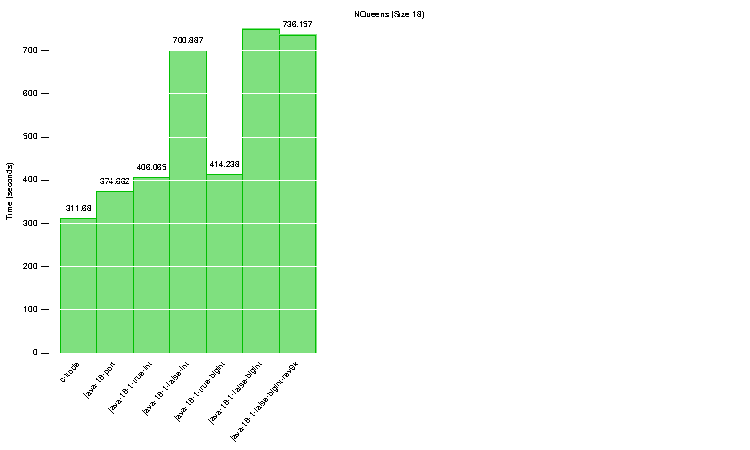
\includegraphics{../benchmarks/lokal.pdf}
\caption{Sammenligning af de lokale test} 
\label{figur:lokal}
\end{center}
\end{figure}

Som det ses er C udgaven en smule hurtigere end den direkte java port, der igen
er lidt hurtigere end den paralleliserede udgave af koden, når den kører
rekursivt. Den iterative udgave er væsentlig langsommere..

Den parallelle udgave af koden er i dette tilfælde her kørt med
\texttt{maxSteps} på 1. 
\begin{figure}[h]
\begin{center}
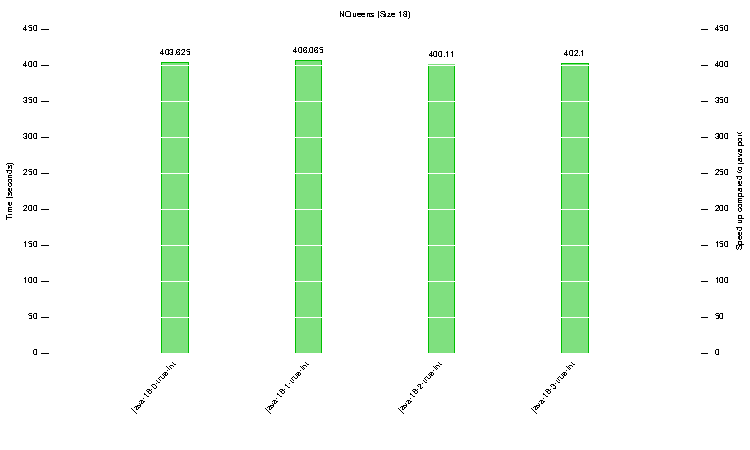
\includegraphics{../benchmarks/maxsteps.pdf}
\caption{insert proper caption here } 
\label{figur:maxsteps}
\end{center}
\end{figure}

På figur \ref{figur:maxsteps} er vist kørsler for $n=18$ for forskellige
$maxSteps$. 
Som det ses, har det ikke den store indflydelse på performance hvor stor
$maxSteps$ er, der er altså ikke det store overhead ved at generere en masse
opgaver og løse dem bagefter, når det kører lokalt. 




I tabel \ref{tabel:noboards} kan det ses hvor mange boards der bliver genereret
for forskellige $n$ og $maxSteps$. 

\fixme{hvor mange jobs bliver der lavet for de forskellige maxsteps, indsæt
tabel?}
\begin{table}
	\begin{center}
		\begin{tabular}{|c|c|c|c|c|c|}
			\hline N  & maxSteps  & boards & n  & maxSteps & boards \\
			\hline 15 & 0         & 18     & 17 & 0        & 21     \\
			\hline 15 & 1         & 173    & 17 & 1        & 243    \\
			\hline 15 & 2         & 1310   & 17 & 2        & 2282   \\ 
			\hline 15 & 3         & 8349   & 17 & 3        & 18161  \\
			\hline 15 & 4         & 43961  & 18 & 0        & 23     \\
			\hline 16 & 0         & 20     & 18 & 1        & 289    \\
			\hline 16 & 1         & 212    & 18 & 2        & 2983   \\
			\hline 16 & 2         & 1797   & 18 & 3        & 26204  \\
			\hline 16 & 3         & 12840  &    &          &        \\
			\hline 16 & 4         & 76224  &    &          &        \\
			\hline
		\end{tabular}
		\caption{Antal Boards der bliver genereret}
		\label{tabel:noboards}
	\end{center}
\end{table}

\begin{table}
	\begin{center}
		\begin{tabular}{|c|c|c|c|}
			\hline N & unikke & totale & totale/unikke \\
			\hline 15 & 285053 & 2279184 & 7.99565 \\
			\hline 16 & 1846955 & 14772512 & 7.99831 \\
			\hline 17 & 11977939 & 95815104  & 7.9993 \\
			\hline 18 & 83263591 & 666090624 & 7.99978 \\
			\hline
		\end{tabular}
		\caption{Antal løsninger}
		\label{tabel:unikkevstotale}
	\end{center}
\end{table}

\begin{figure}[h]
\begin{center}
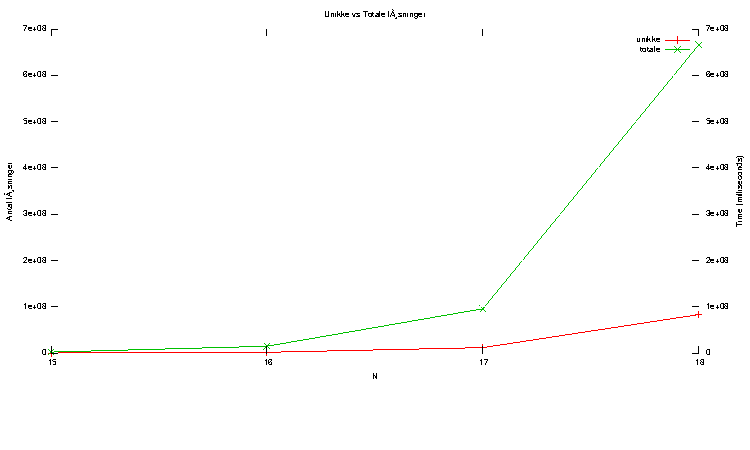
\includegraphics{../benchmarks/unikkevstotale.pdf}
\caption{Unikke og totale antal løsninger} 
\label{figur:unikkevstotale}
\end{center}
\end{figure}

De foregående tests er kørt med kode der bruger \texttt{int} til at gemme resultaterne,
i de næste tests er \texttt{int} skiftet ud med \texttt{BigInteger} 
Her er den rekursive test kørt på revision 83, og den iterative er kørt på
revision 9x. At den iterative er kørt på en anden revision skyldes at der i den
iterative kode var en debug linje der ikke var blevet kommenteret ud, der gjorde
at koden kørte utroligt langsomt.

Som det kan ses på figur \ref{figur:lokal} kører den rekursive kode en smule
langsommere med \texttt{BigInteger} end med \texttt{int}, hvor tiden stiger fra
406.065 til 414.238, hvilket svarer til en forøgelse
på knap 2\% \fixme{hva' med den iterative}


\subsection{kald til backtrack}

Hvis man ser på antallet af kald til backtrack de forskellige versioner laver,
er de ens for c koden og den direkte java port, og hvis man kører med
$maxSteps=0$ er antallet af kald for den parallele og iterative kode også det
samme som for c koden (se tabel \ref{tabel:backtrackkald}. Med $maxSteps>0$ får
vi færre kald til backtrack, hvilket skyldes at en del af disse kald bliver
lavet i forbindelse med oprettelsen af de ekstra boards. 
\fixme{Definition af antal af iterationer er antal kald til den rekursive, og antal løkke-iterationer i den iterative. Det er muligvis interressant pga. performance forklaring.}
\begin{table}
\begin{center}
\begin{tabular}{|c|c|c|}
\hline kodebase  & hjørnebrædt & midtebrædt \\
\hline C kode    &  748267           &  5293206           \\
\hline Java      &  748267           &  5293206           \\
\hline Java rek. &  748267           &  5293206           \\
\hline Java ite. &  748267           &  5293206           \\
\hline
\end{tabular}
\caption{Kald til backtrack for $n=14$}
\label{table:backtrackkald}
\end{center}
\end{table}

\subsection{Jobstørrelse}

Med jobstørrelse refererer vi til hvor lang tid det tager at løse et job, og
ikke størrelsen på data. 
Som det ses i \ref{tabel:jobsize}, varierer jobstørrelsen
meget. Cornerboards er generelt ret små, mens middleboards er generelt er en del
større. Det ses også i tabellen at jobstørrelsen afhænger af de bounds der er i
henholdsvist MiddleBoard og CornerBoard. Hvis man øger $maxSteps$ og dermed får
lavet flere jobs, ses det at de enkelte jobs bliver delt op i nogenlunde lige
støre dele, den relative størrelse mellem det mindste og største jobs er dog
stadig nogenlunde det samme. \fixme{lav en benchmark/beregning der viser dette?}
\fixme{Antallet af jobs er gentagelse fra 1.3/1.4}
\subsection{Generering af jobs}

Det skal bemærkes at indsendelse af jobs afhænger af nethastigheden. De forskellige jobs vi har
submitted til \mig\ har genereringen og indsendelse af jobs svinget fra xx til
xx (se tabel \ref{tabel:jobgenerering}) \fixme{lav den fscking tabel og skriv de
rigtige tal ind}. Langt den største del af tiden går også med at sende jobsne,
da genereringen af jobs for større mængder jobs tager ca 0.01ms/job
\begin{table}
\begin{center}
\begin{tabular}{|c|c|c|c|c|}
\hline N & maxSteps & tid (ms) & brædt & tid (ms) /brædt \\
\hline 17 & 0 & 4 & 21 & 0.19 \\
\hline 17 & 1 & 6 & 243 & 0.02 \\
\hline 17 & 2 & 23 & 2282 & 0.01 \\
\hline 17 & 3 & 206 & 18161 & 0.01 \\
\hline 17 & 4 & 1252 & 121116 & 0.01 \\
\hline 18 & 0 & 4 & 23 & 0.17 \\
\hline 18 & 1 & 6 & 239 & 0.02 \\
\hline 18 & 2 & 44 & 2983 & 0.01 \\
\hline 18 & 3 & 280 & 26204 & 0.01 \\
\hline
\end{tabular}
\caption{Tid for generering af brædt}
\label{table:boardgenering}
\end{center}
\end{table}
\fixme{lav det om til en tabel.. der}

\subsection{Kørsel på \mig}

Den reelle køretid på \mig findes ved at tage \texttt{Queued} tiden for det første job der er
blevet sat i kø, og \texttt{Finished} tiden for det sidste job der er blevet
færdigt, og så finde forskellen.
\fixme{Det ikke interessant at finde køretiden for den første Queued til den sidste Finished.}
På figur \ref{figur:mig} kan man se hvor lang beregningstiden er og hvor lang
den reelle køretid er for $n=18$ og $maxSteps=0,1$. Ved $maxSteps=0$ ses det at
den reelle køretid er næsten det dobbelte af beregningstiden. Når $maxSteps$
bliver sat op til 1 og der dermed bliver genereret flere jobs, kommer der et
noget større overhead, som det kan ses på figuren. På figuren ses det også at
den reelle køretid for den iterative udgave er væsentlig højere end for den
rekursive udgave. Dette skyldes at der har været sat 2 forskellige tests igang
på samme tid, og nogle af de jobs fra den pågældende test er blevet stoppet og
sat i kø igen. De er dermed kommet bagest i køen og først blevet kørt efter den
anden test er færdig. 
\fixme{beregn forholdet mellem den første og resten?}

\begin{figure}[h]
\begin{center}
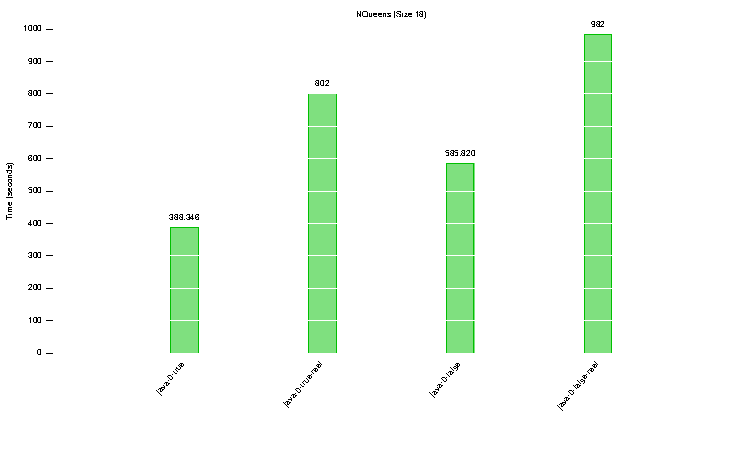
\includegraphics{../benchmarks/mig.pdf}
\caption{NQueen kørt på \mig, for $n=18$ og $maxSteps=0,1$, true er den
rekursive udgave og false den iterative. Reel står for tiden fra det første job
blev queued til det sidste job er finished}
\label{figur:mig}
\end{center}
\end{figure}



\subsubsection{Overhead ved jobskifte}

I MiG\_main() metoden i NQueenJob laver vi et timestamp i starten og slutningen
af metoden.  og kan så tage start tiden for et job og trække sluttiden for det
foregående job fra, og man har så et estimat for hvor lang tid et jobskifte
tager, vi har gjort dette for 8 jobs, og får så 7 estimater, gennemsnittet af
dem bliver 18.455 sek.  Op til 15 af disse 18 sekunder, skyldes at oneclick
applet'en sover i 15 sekunder.  Ved en kørsel med $n=18$ og $maxSteps=1$, hvor
vi så får 289 jobs, giver det knap 89 minutter ved kørsel på én ressource. En del af dette overhead vil
selvfølgelig blive "gemt", når der er flere ressourcer der kører samtidigt.

